%\documentclass[oribibl,a4paper,envcountsame]{llncs}
\documentclass[a4paper]{article}
\setlength\overfullrule{2mm}

\usepackage{listings}

\usepackage{amsmath,amssymb,todonotes,comment}
\usepackage[utf8]{inputenc}
\usepackage{tikz}

\usepackage{algorithm}
\usepackage{algpseudocode}

\usepackage{xcolor,colortbl}
\definecolor{linkcolor}{rgb}{0.65,0,0}
\definecolor{citecolor}{rgb}{0,0.65,0}
\definecolor{urlcolor}{rgb}{0,0,0.65}
\usepackage[colorlinks=true, linkcolor=linkcolor, urlcolor=urlcolor, citecolor=citecolor]{hyperref}

\usepackage{geometry}

\usepackage[british]{babel}
\addto{\captionsbritish}{\renewcommand\abstractname{Abstract.}}

\usepackage{listings}
\lstset{% general command to set parameter(s)
basicstyle=\tiny, % print whole listing small
keywordstyle=\color{black}\bfseries\underbar,
% underlined bold black keywords
identifierstyle=, % nothing happens
commentstyle=\color{white}, % white comments
stringstyle=\ttfamily, % typewriter type for strings
showstringspaces=false} % no special string spaces

\definecolor{mGreen}{rgb}{0,0.6,0}
\definecolor{mGray}{rgb}{0.5,0.5,0.5}
\definecolor{mPurple}{rgb}{0.58,0,0.82}
% \definecolor{backgroundColour}{rgb}{0.95,0.95,0.92}
\definecolor{backgroundColour}{rgb}{0.99,0.99,0.95}

\title{Rescue-Prime Optimized}

%\author{Tomer Ashur$^1$ \and Willi Meier$^2$ \and Alan Szepieniec$^3$ \and Bobbin Threadbare$^4$ \and Al Kindi}

\author{
\begin{tabular}{c}Tomer Ashur$^1$ \\ \small \texttt{tomer.ashur@?} \\ \small ?? \end{tabular}
\begin{tabular}{c}Al Kindi$^2$ \\ \small \texttt{al.kindi@protonmail.com} \\ \small Polygon \end{tabular}
\begin{tabular}{c}Willi meier$^3$ \\ \small \texttt{willi.meier@fhnw} \\ \small FHNW \end{tabular} \\ \\
\begin{tabular}{c}Alan Szepieniec$^4$ \\ \small \texttt{alan@asdm.gmbh} \\ \small AS Discrete Mathematics GmbH \end{tabular}
\begin{tabular}{c}Bobbin Threadbare$^3$ \\ \small \texttt{bobbinth@polygon.technology} \\ \small Polygon \end{tabular} 
}

\begin{document}
\maketitle

\section{Introduction}

This note specifies two instances of a hash function obtained from tailoring Rescue-Prime to a specific context. The context in question is native hashing in a STARK~\cite{cryptoeprint:2018/046} Virtual Machine such as Miden~\cite{miden}.

This context induces unique design constraints, which this specification addresses. The hash function must be defined over the same field that the VM is defined over, which is the prime field with  $p = 2^{64} - 2^{32} + 1$ elements. One of the main use cases is Merkle tree hashing, and so the hash function must support an interface for efficient two-to-one hashing. There are two parameter sets, targeting security level 128 and 160, respectively. 

\section{Specification}

The starting point is Rescue-Prime~\cite{cryptoeprint:2020/1143}, and we assume the reader is familiar with this docment. What is described here is the deviations from this standard. A complete reference implementation in SageMath serves a companion to this specification. It is available at \url{https://github.com/ASDiscreteMathematics/rpo}.

\subsection{Integer Parameters}

\begin{table}[!htp]
\centering
\caption{Integer parameters for the two instances of Rescue-Prime Optimized}
\label{table:integer-parameters}

\begin{tabular}{l||c|c}
prime field modulus $p$ & $2^{64} - 2^{32} + 1$ & $2^{64} - 2^{32} + 1$ \\
security level $\lambda$ & 128 & 160 \\
round number $N$ & 7 & 7 \\
state size $m$ & 12 & 16 \\
rate $r$ & 8 & 10 \\
capacity $c$ & 4 & 6 \\
\end{tabular}
\end{table}

Table~\ref{table:integer-parameters} fixes some integer parameters. Additionally, this choice for $p$ fixes $\alpha$ and $\alpha^{-1}$, which are the exponents of the power maps in the forward and backward S-box layer, respectively (see Fig.~\ref{figure:new-vs-old-half-round}). Specifically, $\alpha = 7$ and
\begin{align*}
\alpha^{-1} &= 10540996611094048183 \\
 &= 1001001001001001001001001001000110110110110110110110110110110111_2 \enspace .
\end{align*}

\subsection{Round Constants}

The round constants are defined as follows:
\begin{itemize}
\item Start from the string \verb@RPO(%i,%i,%i,%i)@.
\item Populate the wildcards ``\texttt{\%i}'' with the ASCII decimal expansion of the integer parameters $p, m, c, \lambda$, in that order.
\item Use SHAKE256 to expand this ASCII string into $9 \cdot 2 \cdot N \cdot m$ pseudorandom bytes.
\item For every chunk of 9 bytes, compute the matching integer by interpreting the byte array as as the integer's base-256 expansion with least significant digit first.
\item Reduce the obtained integer modulo $p$.
\item Collect all such integers. The list of obtained field elements constitutes the list of round constants.
\end{itemize}

The function \texttt{get\_round\_constants} of the reference implementation accomplishes this task.

\subsection{MDS Matrix}

The MDS matrix is circulant. Its first row is $[7, 23, 8, 26, 13, 10, 9, 7, 6, 22, 21, 8]$ for 128 bits of security, and 
$$ [256, 2, 1073741824, 2048, 16777216, 128, 8, 16, 524288, 4194304, 1, 268435456, 1, 1024, 2, 8192] $$
for 160.

\subsection{Order of Operations within a Round}

The operations within every half-round are reordered. The correct order is now: \begin{enumerate}
\item MDS matrix
\item injection of constants
\item alpha or alpha-inverse S-box layer.
\end{enumerate}

\begin{figure}[!htp]
\centering
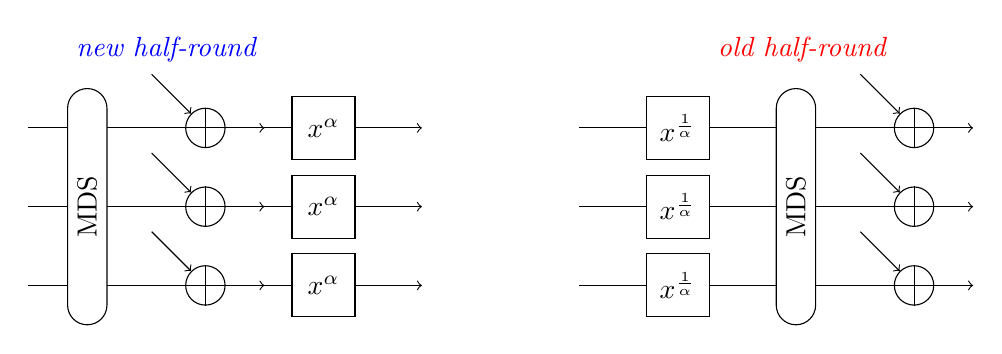
\begin{tikzpicture}

\draw[->] (-0.75, 1) -- (1.25, 1) {};
\draw[->] (-0.75, 0) -- (1.25, 0) {};
\draw[->] (-0.75, -1) -- (1.25, -1) {};
\draw[->] (3.25, 1) -- (8.25, 1) {};
\draw[->] (3.25, 0) -- (8.25, 0) {};
\draw[->] (3.25, -1) -- (8.25, -1) {};

\node[minimum width=0.8cm, minimum height=0.8cm, draw, fill=white] (sbox a) at (0, 1) {$x^{\alpha}$};
\node[minimum width=0.8cm, minimum height=0.8cm, draw, fill=white] (sbox b) at (0, 0) {$x^{\alpha}$};
\node[minimum width=0.8cm, minimum height=0.8cm, draw, fill=white] (sbox b) at (0, -1) {$x^{\alpha}$};

\node[minimum width=0.8cm, minimum height=0.8cm, draw, fill=white] (sbox a) at (4.5, 1) {$x^{\frac{1}{\alpha}}$};
\node[minimum width=0.8cm, minimum height=0.8cm, draw, fill=white] (sbox b) at (4.5, 0) {$x^{\frac{1}{\alpha}}$};
\node[minimum width=0.8cm, minimum height=0.8cm, draw, fill=white] (sbox c) at (4.5, -1) {$x^{\frac{1}{\alpha}}$};

\node[draw, rounded corners=0.25cm, minimum width=3cm, minimum height=0.5cm, rotate=90, fill=white] (mds) at (6, 0) {MDS};

\node[minimum width=0.5cm, minimum height=0.5cm, draw, circle, fill=white] (plus a) at (7.5, 1) {}; \draw[-] (plus a.north) -- (plus a.south) {}; \draw[-] (plus a.east) -- (plus a.west) {}; \draw[->] ([xshift=-0.5cm, yshift=0.5cm] plus a.north west) -- (plus a) {};
\node[minimum width=0.5cm, minimum height=0.5cm, draw, circle, fill=white] (plus b) at (7.5, 0) {}; \draw[-] (plus b.north) -- (plus b.south) {}; \draw[-] (plus b.east) -- (plus b.west) {}; \draw[->] ([xshift=-0.5cm, yshift=0.5cm] plus b.north west) -- (plus b) {};
\node[minimum width=0.5cm, minimum height=0.5cm, draw, circle, fill=white] (plus c) at (7.5, -1) {}; \draw[-] (plus c.north) -- (plus c.south) {}; \draw[-] (plus c.east) -- (plus c.west) {}; \draw[->] ([xshift=-0.5cm, yshift=0.5cm] plus c.north west) -- (plus c) {};

\draw[->] (-3.75, 1) -- (-0.75, 1) {};
\draw[->] (-3.75, 0) -- (-0.75, 0) {};
\draw[->] (-3.75, -1) -- (-0.75, -1) {};

\node[draw, rounded corners=0.25cm, minimum width=3cm, minimum height=0.5cm, rotate=90, fill=white] (mds) at (-3, 0) {MDS};

\node[minimum width=0.5cm, minimum height=0.5cm, draw, circle, fill=white] (plus a) at (-1.5, 1) {}; \draw[-] (plus a.north) -- (plus a.south) {}; \draw[-] (plus a.east) -- (plus a.west) {}; \draw[->] ([xshift=-0.5cm, yshift=0.5cm] plus a.north west) -- (plus a) {};
\node[minimum width=0.5cm, minimum height=0.5cm, draw, circle, fill=white] (plus b) at (-1.5, 0) {}; \draw[-] (plus b.north) -- (plus b.south) {}; \draw[-] (plus b.east) -- (plus b.west) {}; \draw[->] ([xshift=-0.5cm, yshift=0.5cm] plus b.north west) -- (plus b) {};
\node[minimum width=0.5cm, minimum height=0.5cm, draw, circle, fill=white] (plus c) at (-1.5, -1) {}; \draw[-] (plus c.north) -- (plus c.south) {}; \draw[-] (plus c.east) -- (plus c.west) {}; \draw[->] ([xshift=-0.5cm, yshift=0.5cm] plus c.north west) -- (plus c) {};

\node[color=red] (old round) at (6.075, 2) {\it old half-round};
\node[color=blue] (new round) at (-2, 2) {\it new half-round};
\end{tikzpicture}
\caption{New versus old half-rounds.}
\label{figure:new-vs-old-half-round}
\end{figure}

\subsection{Padding Rule}

The padding rule makes a distinction depending on whether the length of the input is a multiple of the rate $r$ or not.
\begin{itemize}
\item If the input length is a multiple of the rate $r$, then initialize the all capacity elements to 0. No preprocessing is applied to the input.
\item If the input length is \emph{not} a multiple of the rate $r$, then append to the input a single 1 element followed by as many zeros as are necessary to make the input length a multiple of the rate. Aditionally, initialize the first capacity element to 1 and all others to 0.
\item The zero-length input is not allowed.
\end{itemize}

In either case the sponge methodology applies: absorb $r$ elements from the input in between applications of the permutation, until no input is left.

\subsection{Overwrite Mode}

In the absorb phase of the sponge construction, the state elements associated with the rate are overwritten by the matching elements from the input chunk, rather than added into. Specifically, if the state elements are $s[0]$ through $s[m-1]$ and the input chunk is $i[0]$ through $i[r-1]$ then correct absorption is given by $s[j] \leftarrow i[j]$ for all $0 \leq j < r$ rather than $s[j] \leftarrow s[j] + i[j]$ for all $0 \leq j < r$.

\subsection{Indexation of State Elements}
\label{section:indexation-spec}

The state is divided into the capacity part, with indices $0$ through $c-1$, and the rate part, with indices $c$ through $m-1$. After the last permutation is done, the digest is given by elements $c$ through $c + r/2 - 1$.

\section{Test Vectors}

The test vectors are generated by the method \texttt{print\_test\_vectors} from the reference implementation. For the sake of completeness, they are repeated here.

\subsection{128 Bits Instance}
\begin{lstlisting}
[0]  -> 
[1502364727743950833 5880949717274681448  162790463902224431 6901340476773664264]

[0 1]  -> 
[ 7478710183745780580  3308077307559720969  3383561985796182409 17205078494700259815]

[0 1 2]  -> 
[17439912364295172999 17979156346142712171  8280795511427637894  9349844417834368814]

[0 1 2 3]  -> 
[ 5105868198472766874 13090564195691924742  1058904296915798891 18379501748825152268]

[0 1 2 3 4]  -> 
[ 9133662113608941286 12096627591905525991 14963426595993304047 13290205840019973377]

[0 1 2 3 4 5]  -> 
[ 3134262397541159485 10106105871979362399   138768814855329459 15044809212457404677]

[0 1 2 3 4 5 6]  ->  
[  162696376578462826  4991300494838863586   660346084748120605 13179389528641752698]

[0 1 2 3 4 5 6 7]  -> 
[ 2242391899857912644 12689382052053305418   235236990017815546  5046143039268215739]

[0 1 2 3 4 5 6 7 8]  -> 
[9585630502158073976 1310051013427303477 7491921222636097758 9417501558995216762]

[0 1 2 3 4 5 6 7 8 9]  -> 
[ 1994394001720334744 10866209900885216467 13836092831163031683 10814636682252756697]

[ 0  1  2  3  4  5  6  7  8  9 10]  -> 
[17486854790732826405 17376549265955727562  2371059831956435003 17585704935858006533]

[ 0  1  2  3  4  5  6  7  8  9 10 11]  -> 
[11368277489137713825  3906270146963049287 10236262408213059745    78552867005814007]

[ 0  1  2  3  4  5  6  7  8  9 10 11 12]  -> 
[17899847381280262181 14717912805498651446 10769146203951775298  2774289833490417856]

[ 0  1  2  3  4  5  6  7  8  9 10 11 12 13]  -> 
[3794717687462954368 4386865643074822822 8854162840275334305 7129983987107225269]

[ 0  1  2  3  4  5  6  7  8  9 10 11 12 13 14]  -> 
[ 7244773535611633983    19359923075859320 10898655967774994333  9319339563065736480]

[ 0  1  2  3  4  5  6  7  8  9 10 11 12 13 14 15]  -> 
[ 4935426252518736883 12584230452580950419  8762518969632303998 18159875708229758073]

[ 0  1  2  3  4  5  6  7  8  9 10 11 12 13 14 15 16]  -> 
[14871230873837295931 11225255908868362971 18100987641405432308  1559244340089644233]

[ 0  1  2  3  4  5  6  7  8  9 10 11 12 13 14 15 16 17]  -> 
[ 8348203744950016968  4041411241960726733 17584743399305468057 16836952610803537051]

[ 0  1  2  3  4  5  6  7  8  9 10 11 12 13 14 15 16 17 18]  -> 
[16139797453633030050  1090233424040889412 10770255347785669036 16982398877290254028]
\end{lstlisting}

\subsection{160 Bits Instance}
\begin{lstlisting}
[0]  -> 
[ 4766737105427868572  7538777753317835226 13644171984579649606  6748107971891460622  3480072938342119934]

[0 1]  -> 
[6277287777617382937 5688033921803605355 1104978478612014217  973672476085279574 7883652116413797779]

[0 1 2]  -> 
[ 3071553803427093579 12239501990998925662 14411295652479845526  5735407824213194294  6714816738691504270]

[0 1 2 3]  -> 
[ 4455998568145007624 18218360213084301612  8963555484142424669 13451196299356019287   660967320761434775]

[0 1 2 3 4]  -> 
[ 7894041400531553560  3138084719322472990 15017675162298246509 12340633143623038238  3710158928968726190]

[0 1 2 3 4 5]  -> 
[18345924309197503617  6448668044176965096  5891298758878861437 18404292940273103487   399715742058360811]

[0 1 2 3 4 5 6]  -> 
[ 4293522863608749708 11352999694211746044 15850245073570756600  1206950096837096206  6945598368659615878]

[0 1 2 3 4 5 6 7]  -> 
[ 1339949574743034442  5967452101017112419   824612579975542151  3327557828938393394 14113149399665697150]

[0 1 2 3 4 5 6 7 8]  -> 
[ 3540904694808418824  5951416386790014715 13859113410786779774 17205554479494520251  7359323608260195110]

[0 1 2 3 4 5 6 7 8 9]  -> 
[ 7504301802792161339 12879743137663115497 17245986604042562042  8175050867418132561  1063965910664731268]

[ 0  1  2  3  4  5  6  7  8  9 10]  -> 
[18267475461736255602  4481864641736940956 11260039501101148638  7529970948767692955  4177810888704753150]

[ 0  1  2  3  4  5  6  7  8  9 10 11]  -> 
[16604116128892623566  1520851983040290492  9361704524730297620  7447748879766268839 10834422028571028806]

[ 0  1  2  3  4  5  6  7  8  9 10 11 12]  -> 
[  243957224918814907  9966149007214472697 18130816682404489504  3814760895598122151   862573500652233787]

[ 0  1  2  3  4  5  6  7  8  9 10 11 12 13]  -> 
[13414343823130474877  1002887112060795246 16685735965176892618 16172309857128312555  5158081519803147178]

[ 0  1  2  3  4  5  6  7  8  9 10 11 12 13 14]  -> 
[14614132925482133961  7618082792229868740  1881720834768448253 11508391877383996679  5348386073072413261]

[ 0  1  2  3  4  5  6  7  8  9 10 11 12 13 14 15]  -> 
[ 6268111131988518030 17920308297240232909 17719152474870950965 14857432101092580778  5708937553833180778]

[ 0  1  2  3  4  5  6  7  8  9 10 11 12 13 14 15 16]  -> 
[11597726741964198121  1568026444559423552  3233218961458461983  9700509409081014876  7989061413164577390]

[ 0  1  2  3  4  5  6  7  8  9 10 11 12 13 14 15 16 17]  -> 
[11180580619692834182 16871004730930134181 17810700669516829599 13679692060051982328 10386085719330760064]

[ 0  1  2  3  4  5  6  7  8  9 10 11 12 13 14 15 16 17 18]  -> 
[ 6222872143719551583  3842704143974291265 18311432727968603639 12278517700025439333  7011953052853282225]
\end{lstlisting}

\section{Motivation}

\subsection{Circulant MDS Matrix}

Rescue-Prime is secure when instantiated with \emph{any} MDS matrix. Therefore, a circulant MDS matrix such as the one proposed by Polygon Zero's may be chosen instead of the one defined by the specification. The obvious questions are
\begin{itemize}
\item[1)] Is the proposed matrix really MDS?
\item[2)] Does the structure enable faster computation of matrix-vector products?
\end{itemize}

As for question (1), we were granted access to Polygon Zero's MDS test procedure and were able to verify the correctness of this function. As a result, we are confident that these circulant matrices specified above are in fact MDS. 

As for question (2), the answer is in the affirmative. Let $R_p = \frac{\mathbb{Z}_p[X]}{\langle X^m - 1\rangle}$ be the ring of polynomials with multiplication modulo $X^m - 1$. There is an isomorphism between the elements of $R_p$ and circulant $m \times m$ matrices over $\mathbb{Z}_p$ given by
\begin{equation}
a_0 + a_1 X + a_2 X^2 + \cdots + a_{m-1} X^{m-1} \leftrightarrow \left( \begin{matrix}
a_0 & a_{m-1} & \cdots & a_1 \\
a_1 & a_0 & & a_2 \\
\vdots & & \ddots & \vdots \\
a_{m-1} & a_{m-2} & \cdots & a_0
\end{matrix} \right) \enspace .
\end{equation}
A fast way to multiply polynomials modulo $X^m - 1$ translates to a fast circulant matrix times vector multiplication procedure.

Note that the coefficient vector of the polynomial corresponds to the first column of the matrix, and not the first row. To translate between row and column, one needs to reverse the entire vector except for the element at the first position.

\subsubsection{Karatsuba-based}

Karatsuba multiplication~\cite{karatsuba1962multiplication} splits the multiplication of two polynomials of degree at most $n-1$ up into three multiplications of polynomials of degree $n/2 - 1$, and applies that split recursively. In the limit the procedure requires only $O(n^{1.58})$ multiplications, compared to the $n^2$ for the schoolbook algorithm. While the number of multiplications is reduced, the number of additions is increased. However, additions generally do not need to be followed up with modular reduction.

Let $a(X) = a_l(X) + X^{n/2} \cdot a_r(X)$ and $b(X) = b_l(X) + X^{n/2} \cdot b_r(X)$ with all of $a_l(X)$, $a_r(X)$, $b_l(X)$, and $b_r(X)$ having degree at most $n/2-1$. Let
\begin{itemize}
\item $c_0(X) = a_l(X) \times a_l(X)$,
\item $c_2(X) = a_r(X) \times b_r(X)$,
\item $c_1(X) = (a_l(X) + a_r(X)) \times (b_l(X) + b_r(X)) - c_0(X) - c_2(X)$;
\end{itemize}
then $c(X) = a(X) \times b(X) = c_0(X) + X^{n/2} \cdot c_1(X) + X^n \cdot c_2(X)$. Note that $c(X)$ can be calculated with only $3$ multiplications of polynomials of half the number of coefficients. Applying this reduction recursively is what generates Karatsuba's multiplication algorithm.

After using Karatsuba to find the product of two polynomials $t(X)$ and $s(X)$ that represent the MDS matrix and state vector respectively, the next step is the reduction modulo $X^m-1$. This step is straightforward: just iterate over the coefficients of monomials $X^{m/2}$ through $X^{m-1}$ and add them to the coefficients of monomials $X^0$ through $X^{m/2-1}$.

\subsubsection{NTT-based}

Using the same isomorphism as in the previous section and the fact that multiplication in the ring $R_p$ can be done efficiently using the Number Theory Transform (NTT) and its inverse, we can get a $O(n \cdot\log(n))$ algorithm for circulant matrix times vector multiplication procedure. More precisely, let $\omega$ be a primitive $n$-th root of unity and define the following ${\mathbb{Z}_p[X]}$-linear map:

\begin{equation}
	NTT_{\omega} :
	\begin{cases}
		R_p \longrightarrow \left({\mathbb{Z}_p}\right)^n\\
		a(X) \mapsto \left(a(\omega^0), a(\omega^1),\cdots, a(\omega^n)\right)
	\end{cases}       
\end{equation}
which is just the evaluation of the polynomial $a$ at the powers of $\omega$, i.e. the $n$-th roots of unity. This is called the \textit{Number Theory Transform} (\textit{NTT}), and is a special case of the Discrete Fourier Transform. Then, using the Chinese Remainder Theorem, one can show that $NTT_{\omega}$ is an isomorphism of algebras. This means that, in particular, the following holds:\[NTT_{\omega}\left(a(X)\times b(X)\right) = NTT_{\omega}(a(X)) \odot  NTT_{\omega}(b(X)) \]
or equivalently \[a(X)\times b(X) = NTT_{\omega}^{-1}\big(NTT_{\omega}(a(X)) \odot  NTT_{\omega}(b(X))\big) \] 
where is $\odot$ is the Hadamard product.
This in particular yields the following algorithm:
\begin{algorithm}
	\caption{Circulant matrix times vector multiplication using NTT}\label{alg:cap}
	\begin{algorithmic}
		\Require $n \geq 1$, $a(X), b(X) \in R_p$ and $\omega$ is a primitive $n$-th root of unity.
		\Ensure $C(X) = a(X)\times b(X)$
		\State $\alpha \gets NTT_{\omega}(a(X))$
		\State $\beta \gets NTT_{\omega}(b(X))$
		\State $\gamma \gets \alpha\odot \beta$
		\State $C(X) \gets  NTT_{\omega}^{-1}\big(\gamma\big)$
	\end{algorithmic}
\end{algorithm}

Given that in our current context the matrix we are multiplying with is fixed once and for all, the previous algorithm can be optimized by pre-computing the NTT of the MDS matrix such that in the end it will be necessary to compute only one NTT and one inverse NTT per input vector $b$. Since the NTT and the inverse NTT can be computed in $O(n \cdot\log(n))$ using the Fast Fourier Transform (FFT), the complexity of Alg.~\ref{alg:cap} is also $O(n \cdot\log(n))$.

\subsection{Reduced Round Number}
\label{section:round-number}

According to the specification~\cite{cryptoeprint:2020/1143}, the Gröbner basis attack dominates for the range in which the given parameters lie. Moreover, the number of rounds should be set to $N = \lceil 1.5 \cdot \min(l_1, 5)\rceil$, where $l_1$ is the minimal number required to guarantee that the Gröbner basis attack has complexity at least as large as the security parameter, and where the factor 1.5 is a security margin.

For both the 128-bit variant and the 160-bit variant, the estimate for the complexity of the Gröbner basis attack exceeds the security level as soon as $N \geq 3$. Plugging this data point into the formula gives rise to a recommended number of rounds of $N = \lceil 1.5 \cdot 5 \rceil = 8$. Setting instead $N=7$ constitutes a 12.5\% reduction in the number of rounds.

The reason why we feel confident recommending $N=7$ is threefold:
\begin{itemize}
 \item The relative reduction is still less than the relative security margin induced by the factor 1.5.
 \item The estimate of the Gröbner basis attack complexity according to the specification is still more than double the security level. The estimate according to experiments run in the course of this research project were lower, but still indicate that the security target is met with margin.
 \item Since the publication of the original Marvellous paper~\cite{cryptoeprint:2019/426}, the first version of which appeared online in 2019, there has been zero progress in attacking either Rescue or Rescue-Prime.
\end{itemize}
 
\subsection{Order of Operations for Better Folding}

On of the costly steps in both the prover and the verifier of a STARK is the computation of the vector of values of AIR transition constraint polynomials for two consecutive rows of the algebraic execution trace (AET). The AIR constraints are evaluated point by point on the codewords that represent the trace. The generated codewords are different from zero except in locations that correspond to a row in the AET and its successor.

Rescue and Rescue-Prime have S-boxes that send $x$ to $x^{\frac{1}{\alpha}}$, where $\alpha$ is the smallest invertible non-trivial power map degree. To avoid a very high degree AIR, the Marvellous paper~\cite{cryptoeprint:2019/426} introduced \emph{folding}. This technique involves arithmetizing the evolution of the state forwards in time for a part of the time step, and backwards in time for the remaining part. By traversing over the $x \mapsto x^{\frac{1}{\alpha}}$ map backwards, the degree of the resulting AIR drops to $\alpha$. The equation is found by equating two distinct expressions for the value of the same wire in the middle. The corresponding polynomial is found by moving all terms to the left hand side.

\begin{figure}[!htp]
\centering
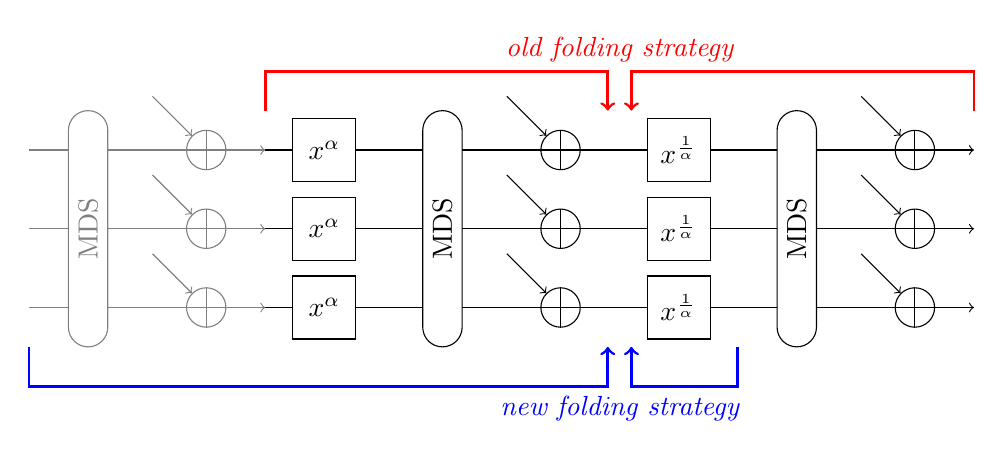
\begin{tikzpicture}

\draw[->] (-0.75, 1) -- (8.25, 1) {};
\draw[->] (-0.75, 0) -- (8.25, 0) {};
\draw[->] (-0.75, -1) -- (8.25, -1) {};

\node[minimum width=0.8cm, minimum height=0.8cm, draw, fill=white] (sbox a) at (0, 1) {$x^{\alpha}$};
\node[minimum width=0.8cm, minimum height=0.8cm, draw, fill=white] (sbox b) at (0, 0) {$x^{\alpha}$};
\node[minimum width=0.8cm, minimum height=0.8cm, draw, fill=white] (sbox b) at (0, -1) {$x^{\alpha}$};

\node[draw, rounded corners=0.25cm, minimum width=3cm, minimum height=0.5cm, rotate=90, fill=white] (mds) at (1.5, 0) {MDS};

\node[minimum width=0.5cm, minimum height=0.5cm, draw, circle, fill=white] (plus a) at (3, 1) {}; \draw[-] (plus a.north) -- (plus a.south) {}; \draw[-] (plus a.east) -- (plus a.west) {}; \draw[->] ([xshift=-0.5cm, yshift=0.5cm] plus a.north west) -- (plus a) {};
\node[minimum width=0.5cm, minimum height=0.5cm, draw, circle, fill=white] (plus b) at (3, 0) {}; \draw[-] (plus b.north) -- (plus b.south) {}; \draw[-] (plus b.east) -- (plus b.west) {}; \draw[->] ([xshift=-0.5cm, yshift=0.5cm] plus b.north west) -- (plus b) {};
\node[minimum width=0.5cm, minimum height=0.5cm, draw, circle, fill=white] (plus c) at (3, -1) {}; \draw[-] (plus c.north) -- (plus c.south) {}; \draw[-] (plus c.east) -- (plus c.west) {}; \draw[->] ([xshift=-0.5cm, yshift=0.5cm] plus c.north west) -- (plus c) {};

\node[minimum width=0.8cm, minimum height=0.8cm, draw, fill=white] (sbox a) at (4.5, 1) {$x^{\frac{1}{\alpha}}$};
\node[minimum width=0.8cm, minimum height=0.8cm, draw, fill=white] (sbox b) at (4.5, 0) {$x^{\frac{1}{\alpha}}$};
\node[minimum width=0.8cm, minimum height=0.8cm, draw, fill=white] (sbox c) at (4.5, -1) {$x^{\frac{1}{\alpha}}$};

\node[draw, rounded corners=0.25cm, minimum width=3cm, minimum height=0.5cm, rotate=90, fill=white] (mds) at (6, 0) {MDS};

\node[minimum width=0.5cm, minimum height=0.5cm, draw, circle, fill=white] (plus a) at (7.5, 1) {}; \draw[-] (plus a.north) -- (plus a.south) {}; \draw[-] (plus a.east) -- (plus a.west) {}; \draw[->] ([xshift=-0.5cm, yshift=0.5cm] plus a.north west) -- (plus a) {};
\node[minimum width=0.5cm, minimum height=0.5cm, draw, circle, fill=white] (plus b) at (7.5, 0) {}; \draw[-] (plus b.north) -- (plus b.south) {}; \draw[-] (plus b.east) -- (plus b.west) {}; \draw[->] ([xshift=-0.5cm, yshift=0.5cm] plus b.north west) -- (plus b) {};
\node[minimum width=0.5cm, minimum height=0.5cm, draw, circle, fill=white] (plus c) at (7.5, -1) {}; \draw[-] (plus c.north) -- (plus c.south) {}; \draw[-] (plus c.east) -- (plus c.west) {}; \draw[->] ([xshift=-0.5cm, yshift=0.5cm] plus c.north west) -- (plus c) {};

\draw[->, color=gray] (-3.75, 1) -- (-0.75, 1) {};
\draw[->, color=gray] (-3.75, 0) -- (-0.75, 0) {};
\draw[->, color=gray] (-3.75, -1) -- (-0.75, -1) {};

\node[draw, rounded corners=0.25cm, minimum width=3cm, minimum height=0.5cm, rotate=90, color=gray, fill=white] (mds) at (-3, 0) {MDS};

\node[minimum width=0.5cm, minimum height=0.5cm, draw, circle, color=gray, fill=white] (plus a) at (-1.5, 1) {}; \draw[-, color=gray] (plus a.north) -- (plus a.south) {}; \draw[-, color=gray] (plus a.east) -- (plus a.west) {}; \draw[->, color=gray] ([xshift=-0.5cm, yshift=0.5cm] plus a.north west) -- (plus a) {};
\node[minimum width=0.5cm, minimum height=0.5cm, draw, circle, color=gray, fill=white] (plus b) at (-1.5, 0) {}; \draw[-, color=gray] (plus b.north) -- (plus b.south) {}; \draw[-, color=gray] (plus b.east) -- (plus b.west) {}; \draw[->, color=gray] ([xshift=-0.5cm, yshift=0.5cm] plus b.north west) -- (plus b) {};
\node[minimum width=0.5cm, minimum height=0.5cm, draw, circle, color=gray, fill=white] (plus c) at (-1.5, -1) {}; \draw[-, color=gray] (plus c.north) -- (plus c.south) {}; \draw[-, color=gray] (plus c.east) -- (plus c.west) {}; \draw[->, color=gray] ([xshift=-0.5cm, yshift=0.5cm] plus c.north west) -- (plus c) {};

\draw[->, color=red, line width=1] (8.25, 1.5) -- (8.25, 2) -- (3.9, 2) -- (3.9, 1.5) {};
\draw[->, color=red, line width=1] (-0.75, 1.5) -- (-0.75, 2) -- (3.6, 2) -- (3.6, 1.5) {};
\node[color=red, anchor=south] (old folding) at (3.75, 2) {\it old folding strategy};

\draw[->, color=blue, line width=1] (-3.75, -1.5) -- (-3.75, -2) -- (3.6, -2) -- (3.6, -1.5) {};
\draw[->, color=blue, line width=1] (5.25, -1.5) -- (5.25, -2) -- (3.9, -2) -- (3.9, -1.5) {};
\node[color=blue, anchor=north] (new folding) at (3.75, -2) {\it new folding strategy};

\end{tikzpicture}
\caption{New versus old folding strategy.}
\end{figure}

The original folding strategy makes no distinction between the cost of multiplying a vector by a matrix or by its inverse. The AIR polynomials have the same number of terms. However, considerable effort was spent making the MDS matrix-vector multiplication fast, and it seems difficult to simultaneously make multiplication by the matrix's inverse fast. This problem motivates an alternative folding strategy, namely one that avoids using the inverse MDS matrix altogether.

The new folding strategy in forwards direction: one MDS, one injection of constants, one $x \mapsto x^\alpha$ S-box layer, another MDS, and another injection of constants. Only the map $x \mapsto ^{\frac{1}{\alpha}}$ is computed in backwards direction.

To argue why this re-arrangement does not affect security, consider moving the MDS matrix and injection of constants of the very last step to the front. This move does not degrade security according to the following heuristic argument. An attack that meaningfully distinguishes the new permutation (that is, after the move) from a permutation selected uniformly at random, can be translated to an attack on the old permutation (that is, before rearrangement) with a linear overhead. Note that the round constants are sampled independently from those of Rescue-Prime.

\subsection{Usability in a Stack-Based Virtual Machine}

\subsubsection{Indexation}

As per \S~\ref{section:indexation-spec}, the capacity elements are indexed $0$ through $c-1$ and the rate elements $c$ through $m-1$. This choice stands in contrast to traditional indexing choices, which puts the rate part first. While the choice of indexation is irrelevant from a security point of view (see below), this present choice benefits usability in the context of a stack machine.

The unorthodox indexing scheme corresponds to putting the capacity part deep into the stack, and the rate part in the shallow end. As a result, squeezing and absorbing corresponds to operations that affect only the top of the stack. The capacity part of the sponge state does not need to be touched except when the hasher is initialized and after hashing is finished.

To see why any choice of indexation is arbitrary from the point of view of security, observe that any permutation can be absorbed into one or even all MDS matrices without changing the fact that they are MDS. The end result is a permutation with an identical security argument.

\subsubsection{Overwrite Mode}

In many stack-based VMs, at most one element can be pushed onto the stack per clock cycle. Therefore, first pushing elements onto the stack and then adding them into the sponge state would require a large number of operations: in addition to push and add operations, stack manipulation operations are also necessary to arrange the stack correctly. In the overwrite mode, we can drop rate elements from the stack and then simply push the new rate elements onto the stack. This procedure is strictly more efficient than the procedure when elements are absorbed through addition as it requires no additional stack manipulation operations.

The alternative of to overwriting the rate part of the sponge that does not blow up the number of cycles, is to introduce a single instruction which adds elements to be absorbed to the top $r$ elements of the stack. This alternative a) require one extra instruction, and b) would make the original elements inaccessible, for instance if they need to be saved to memory. For example, to invert a hash non-deterministically, one might like to do something like this:

\begin{enumerate}

\item Absorb $r$ into the top of the stack.
\item Save the top $r$ stack elements to memory.
\item Apply the Rescue-XLIX permutation to the top $m$ elements of the stack.

\end{enumerate}

If in step (1) elements are absorbed through addition rather than overwriting, step (2) becomes impossible.

The security of overwrite mode has been analyzed e.g. in \S~4.3 of the Sponge SoK~\cite{sponge}.

\subsection{Padding Rule}

\vspace{0.25cm}
\textsc{Acknowledgments} This project was made possible through the financial support of \href{https://polygon.technology/}{Polygon}, for which the authors would like to express gratitude.


\bibliographystyle{plain}
\bibliography{bib}

\end{document}

